\documentclass[12pt, titlepage]{article}

\usepackage{fullpage}
\usepackage[round]{natbib}
\usepackage{multirow}
\usepackage{booktabs}
\usepackage{tabularx}
\usepackage{graphicx}
\usepackage{float}
\usepackage{hyperref}
\hypersetup{
    colorlinks,
    citecolor=blue,
    filecolor=black,
    linkcolor=red,
    urlcolor=blue
}

%%% Comments

\usepackage{color}

\newif\ifcomments\commentstrue %displays comments
%\newif\ifcomments\commentsfalse %so that comments do not display

\ifcomments
\newcommand{\authornote}[3]{\textcolor{#1}{[#3 ---#2]}}
\newcommand{\todo}[1]{\textcolor{red}{[TODO: #1]}}
\else
\newcommand{\authornote}[3]{}
\newcommand{\todo}[1]{}
\fi

\newcommand{\wss}[1]{\authornote{blue}{SS}{#1}} 
\newcommand{\plt}[1]{\authornote{magenta}{TPLT}{#1}} %For explanation of the template
\newcommand{\an}[1]{\authornote{cyan}{Author}{#1}}
 % CHANGE BACK
%% Comments

\usepackage{color}

\newif\ifcomments\commentstrue %displays comments
%\newif\ifcomments\commentsfalse %so that comments do not display

\ifcomments
\newcommand{\authornote}[3]{\textcolor{#1}{[#3 ---#2]}}
\newcommand{\todo}[1]{\textcolor{red}{[TODO: #1]}}
\else
\newcommand{\authornote}[3]{}
\newcommand{\todo}[1]{}
\fi

\newcommand{\wss}[1]{\authornote{blue}{SS}{#1}} 
\newcommand{\plt}[1]{\authornote{magenta}{TPLT}{#1}} %For explanation of the template
\newcommand{\an}[1]{\authornote{cyan}{Author}{#1}}
 % CHANGE BACK
%%% Common Parts

\newcommand{\progname}{ProgName} % PUT YOUR PROGRAM NAME HERE
\newcommand{\authname}{Team \#, Team Name
\\ Student 1 name
\\ Student 2 name
\\ Student 3 name
\\ Student 4 name} % AUTHOR NAMES                  

\usepackage{hyperref}
    \hypersetup{colorlinks=true, linkcolor=blue, citecolor=blue, filecolor=blue,
                urlcolor=blue, unicode=false}
    \urlstyle{same}
                                
 % CHANGE BACK
%% Common Parts

\newcommand{\progname}{ProgName} % PUT YOUR PROGRAM NAME HERE
\newcommand{\authname}{Team \#, Team Name
\\ Student 1 name
\\ Student 2 name
\\ Student 3 name
\\ Student 4 name} % AUTHOR NAMES                  

\usepackage{hyperref}
    \hypersetup{colorlinks=true, linkcolor=blue, citecolor=blue, filecolor=blue,
                urlcolor=blue, unicode=false}
    \urlstyle{same}
                                
 

\newcounter{acnum}
\newcommand{\actheacnum}{AC\theacnum}
\newcommand{\acref}[1]{AC\ref{#1}}

\newcounter{ucnum}
\newcommand{\uctheucnum}{UC\theucnum}
\newcommand{\uref}[1]{UC\ref{#1}}

\newcounter{mnum}
\newcommand{\mthemnum}{M\themnum}
\newcommand{\mref}[1]{M\ref{#1}}

\begin{document}

\title{Module Guide for \progname{}} 
\author{\authname}
\date{\today}

\maketitle

\pagenumbering{roman}

\section{Revision History}

\begin{tabularx}{\textwidth}{llX}
\textbf{Date} & \textbf{Developer(s)} & \textbf{Change}\\
\midrule
18/01/2023 & Namit Chopra, Brandon Duong & Finished first version \\
 & Andrew Balmakund, Mohammad Harun \\
 & Mihail Serafimovski & \\
 04/03/2023 & Namit Chopra, Brandon Duong & Finished second version \\
 & Andrew Balmakund, Mohammad Harun \\
 & Mihail Serafimovski & \\
 04/05/2023 & Namit Chopra, Brandon Duong & Addressed GitHub issues \\
 & Andrew Balmakund, Mohammad Harun \\
 & Mihail Serafimovski & \\
 % & Andrew Balmakund, Mohammad Harun \\
 % & Mihail Serafimovski & \\
\bottomrule
\end{tabularx}

\newpage

\section{Reference Material}

This section records information for easy reference.

\subsection{Abbreviations and Acronyms}

\renewcommand{\arraystretch}{1.2}
\begin{tabular}{l l} 
  \toprule		
  \textbf{symbol} & \textbf{description}\\
  \midrule 
  AC & Anticipated Change\\
  DAG & Directed Acyclic Graph \\
  M & Module \\
  MG & Module Guide \\
  OS & Operating System \\
  FR & Functional Requirement\\
  NR & Non-Functional Requirement\\
  LF & Look and Feel Requirement\\
  UH & Usability and Humanity Requirement\\
  PR & Performance Requirement\\
  OE & Operations and Environmental Requirement\\
  MR & Maintainability and Support Requirement\\
  SR & Security Requirement\\
  LR & Legal Requirement\\
  SC & Scientific Computing \\
  SRS & Software Requirements Specification\\
  UI & User Interface\\
  \progname & Final Year Software Engineering Capstone Project name\\
  UC & Unlikely Change \\
  \bottomrule
\end{tabular}\\

\newpage

\tableofcontents

\listoftables

\listoffigures

\newpage

\pagenumbering{arabic}

\section{Introduction}

Decomposing a system into modules is a commonly accepted approach to developing
software.  A module is a work assignment for a programmer or programming
team (Parnas et al., 1984).  We advocate a decomposition
based on the principle of information hiding (Parnas et al., 1972).  This principle supports design for change because the ``secrets'' that each module hides represent likely future changes.  Design for change is valuable in SC, where modifications are frequent, especially during initial development as the solution space is explored.

Our design follows the rules laid out by Parnas as follows:
\begin{itemize}
\item System details that are likely to change independently should be the
  secrets of separate modules.
\item Each data structure is implemented in only one module.
\item Any other program that requires information stored in a module's data
  structures must obtain it by calling access programs belonging to that module.
\end{itemize}

After completing the first stage of the design, the Software Requirements
Specification (SRS), the Module Guide (MG) is developed (Parnas et al., 1984). The MG specifies the modular structure of the system and is intended to allow both designers and maintainers to easily identify the parts of the software.  The potential readers of this document are as follows:

\begin{itemize}
\item New project members: This document can be a guide for a new project member
  to easily understand the overall structure and quickly find the
  relevant modules they are searching for.
\item Maintainers: The hierarchical structure of the module guide improves the
  maintainers' understanding when they need to make changes to the system. It is
  important for a maintainer to update the relevant sections of the document
  after changes have been made.
\item Designers: Once the module guide has been written, it can be used to
  check for consistency, feasibility, and flexibility. Designers can verify the
  system in various ways, such as consistency among modules, the feasibility of the
  decomposition, and flexibility of the design.
\end{itemize}

The rest of the document is organized as follows. Section
\ref{SecChange} lists the anticipated and unlikely changes in the software
requirements. Section \ref{SecMH} summarizes the module decomposition that
was constructed according to the likely changes. Section \ref{SecConnection}
specifies the connections between the software requirements and the
modules. Section \ref{SecMD} gives a detailed description of the
modules. Section \ref{SecTM} includes two traceability matrices. One checks
the completeness of the design against the requirements provided in the SRS. The
other shows the relation between anticipated changes and the modules. Section
\ref{SecUse} describes the use relation between modules.

\section{Anticipated and Unlikely Changes} \label{SecChange}

This section lists possible changes to the system. According to the likeliness
of the change, the possible changes are classified into two
categories. Anticipated changes are listed in Section \ref{SecAchange}, and
unlikely changes are listed in Section \ref{SecUchange}.

\subsection{Anticipated Changes} \label{SecAchange}

Anticipated changes are the source of the information that is to be hidden
inside the modules. Ideally, changing one of the anticipated changes will only
require changing the one module that hides the associated decision. The approach
adopted here is called design for
change.

\begin{description}
\item[\refstepcounter{acnum} \actheacnum \label{PriceFluctuate}:] Fluctuating prices for purchasing an item
\item[\refstepcounter{acnum} \actheacnum \label{AvatarVariety}:] Adding more variety to the type of avatars for the user to interact with
\item[\refstepcounter{acnum} \actheacnum \label{ItemVariety}:] Adding more items in the shop
\item[\refstepcounter{acnum} \actheacnum \label{EventMechanism}:] The effects of natural disasters on the farm grid
\item[\refstepcounter{acnum} \actheacnum \label{ConsultantMechanism}:] The method for determining the likelihood of future events for the consultant
\item[\refstepcounter{acnum} \actheacnum \label{SoundtrackVariety}:] Multiple soundtracks for different aspects of the game
\item[\refstepcounter{acnum} \actheacnum \label{SellOptions}:] The method to sell harvested crops 
\item[\refstepcounter{acnum} \actheacnum \label{PurchaseInsurance}:] The method to buy insurance for a purchased item
\item[\refstepcounter{acnum} \actheacnum \label{InsuranceAlgorithm}:] The statistical technique utilized for the insurance system
\item[\refstepcounter{acnum} \actheacnum \label{UIComponents}:] The user interface layout of the game
\item[\refstepcounter{acnum} \actheacnum \label{SaveGame}:] The method of saving game state
\item[\refstepcounter{acnum} \actheacnum \label{TurnNumber}:] The number of turns per season


\end{description}

\subsection{Unlikely Changes} \label{SecUchange}

The module design should be as general as possible. However, a general system is
more complex. Sometimes this complexity is not necessary. Fixing some design
decisions at the system architecture stage can simplify the software design. If
this decision should later need to be changed, then many parts of the design
will potentially need to be modified. Hence, it is not intended that these
decisions will be changed.

\begin{description}
\item[\refstepcounter{ucnum} \uctheucnum \label{ucIO}:] User input for the in-game controls
\item [\refstepcounter{ucnum} \uctheucnum \label{ucIO}:] The details needed to create an account
\item [\refstepcounter{ucnum} \uctheucnum \label{ucIO}:] The environment in which the user will be able to play the game
\item [\refstepcounter{ucnum} \uctheucnum \label{ucIO}:] The system will only one login session per user
\item [\refstepcounter{ucnum} \uctheucnum \label{ucIO}:] The specific game data collected for research
\item [\refstepcounter{ucnum} \uctheucnum \label{ucIO}:] The ability to purchase and sell items
\item [\refstepcounter{ucnum} \uctheucnum \label{ucIO}:] The ability to access a consultant 
\item [\refstepcounter{ucnum} \uctheucnum \label{ucIO}:] The authentication of a user is required before performing actions in the game 
\item [\refstepcounter{ucnum} \uctheucnum \label{ucIO}:] The ability to delete user data
\item [\refstepcounter{ucnum} \uctheucnum \label{ucIO}:] The ability to plant and harvest a crop
\item [\refstepcounter{ucnum} \uctheucnum \label{ucIO}:] The changing of seasons


\end{description}

\section{Module Hierarchy} \label{SecMH}

This section provides an overview of the module design. Modules are summarized
in a hierarchy decomposed by secrets in Table \ref{TblMH}. The modules listed
below, which are leaves in the hierarchy tree, are the modules that will
be implemented.

\begin{description}
\item [\refstepcounter{mnum} \mthemnum \label{GenerateStatistic}:] GenerateStatistic
\item [\refstepcounter{mnum} \mthemnum \label{Avatar}:] Avatar
\item [\refstepcounter{mnum} \mthemnum \label{AvatarMenu}:] AvatarMenu
\item [\refstepcounter{mnum} \mthemnum \label{Consultant}:] Consultant
\item [\refstepcounter{mnum} \mthemnum \label{OtherAvatar}:] OtherAvatar
\item [\refstepcounter{mnum} \mthemnum \label{SeasonalEvents}:] SeasonalEvents
\item [\refstepcounter{mnum} \mthemnum \label{Item}:] Item
\item [\refstepcounter{mnum} \mthemnum \label{Inventory}:] Inventory
\item [\refstepcounter{mnum} \mthemnum \label{Shop}:] Shop
\item [\refstepcounter{mnum} \mthemnum \label{DatabaseOperations}:] DatabaseOperations
\item [\refstepcounter{mnum} \mthemnum \label{MusicPlayer}:] MusicPlayer
\item [\refstepcounter{mnum} \mthemnum \label{GameSettings}:] GameSettings
\item [\refstepcounter{mnum} \mthemnum \label{AuthState}:] AuthState
\item [\refstepcounter{mnum} \mthemnum \label{Socket}:] Socket
\item [\refstepcounter{mnum} \mthemnum \label{ClientFirebase}:] ClientFirebase
\item [\refstepcounter{mnum} \mthemnum \label{User}:] User
\item [\refstepcounter{mnum} \mthemnum \label{AuthError}:] AuthError
\item [\refstepcounter{mnum} \mthemnum \label{CreateAccount}:] CreateAccount
\item [\refstepcounter{mnum} \mthemnum \label{Login}:] Login
\item [\refstepcounter{mnum} \mthemnum \label{ServerFirebase}:] ServerFirebase
\item [\refstepcounter{mnum} \mthemnum \label{RedisClient}:] RedisClient
\item [\refstepcounter{mnum} \mthemnum \label{Server}:] Server
\item [\refstepcounter{mnum} \mthemnum \label{Seed}:] Seed
\item [\refstepcounter{mnum} \mthemnum \label{FarmTile}:] FarmTile
\item [\refstepcounter{mnum} \mthemnum \label{FarmGrid}:] FarmGrid
\item [\refstepcounter{mnum} \mthemnum \label{GameController}:] GameController
\end{description}


\begin{table}[H]
\centering
\begin{tabular}{p{0.3\textwidth} p{0.6\textwidth}}
\toprule
\textbf{Level 1} & \textbf{Level 2}\\
\midrule

{Hardware-Hiding Module} & - \\
\midrule

\multirow{10}{0.3\textwidth}{Behaviour-Hiding Module} & GameController\\
& AvatarMenu\\
& Shop\\
& Inventory\\
& FarmGrid\\
& GameSettings\\
& CreateAccount\\
& Login\\
& SeasonalEvents\\
& GenerateStatistic\\
\midrule

\multirow{18}{0.3\textwidth}{Software-Hiding Module} & Avatar\\
& Consultant\\
& OtherAvatars\\
& FarmTile\\
& Seed\\
& Item\\
& DatabaseOperations\\ 
& ServerFirebase\\
& ClientFirebase\\
& AuthState\\
& Socket\\
& RedisClient\\
& Server\\ 
& MusicPlayer \\
& User \\
& AuthError \\
\bottomrule

\end{tabular}
\caption{Module Hierarchy}
\label{TblMH}
\end{table}

\section{Connection Between Requirements and Design} \label{SecConnection}

The design of the system is intended to satisfy the requirements developed in
the SRS. In this stage, the system is decomposed into modules. The connection
between requirements and modules is listed in Table~\ref{TblRT}.

\section{Module Decomposition} \label{SecMD}

Modules are decomposed according to the principle of ``information hiding''
proposed by \citet{ParnasEtAl1984}. The \emph{Secrets} field in a module
decomposition is a brief statement of the design decision hidden by the
module. The \emph{Services} field specifies \emph{what} the module will do
without documenting \emph{how} to do it. For each module, a suggestion for the
implementing software is given under the \emph{Implemented By} title. If the
entry is \emph{OS}, this means that the module is provided by the operating
system or by standard programming language libraries.  \emph{\progname{}} means the
module will be implemented by the \progname{} software.

Only the leaf modules in the hierarchy have to be implemented. If a dash
(\emph{--}) is shown, this means that the module is not a leaf and will not have
to be implemented. 

\subsection{Hardware Hiding Modules }

\begin{description}
\item[Secrets:]The data structure and the algorithm used to implement the virtual
  hardware.
\item[Services:]Serves as virtual hardware used by the rest of the
  system. This module provides the interface between the hardware and the
  software. So, the system can use it to display outputs or to accept inputs.
\item[Implemented By:] OS
\end{description}

\subsection{Behaviour-Hiding Module}

\begin{description}
\item[Secrets:]The contents of the required behaviors.
\item[Services:]Includes programs that provide externally visible behavior of
  the system as specified in the software requirements specification (SRS)
  documents. This module serves as a communication layer between the
  hardware-hiding module and the software decision module. The programs in this
  module will need to change if there are changes in the SRS.
\item[Implemented By:] --
\end{description}


\subsubsection{GameController (\mref{GameController})}

\begin{description}
\item[Secrets:] User input handlers and in-game logic.
\item[Services:] Responsible for calling all related submodules throughout a session.
\item[Implemented By:]  \progname
\item[Type of Module:] Library
\end{description}

\subsubsection{AvatarMenu (\mref{AvatarMenu})}

\begin{description}
\item[Secrets:] User input handling during the menu.
\item[Services:] Interact with the user selecting several avatars to choose to interact with.
\item[Implemented By:]  \progname
\item[Type of Module:] Library
\end{description}


\subsubsection{Shop (\mref{Shop})}

\begin{description}
\item[Secrets:] The data structure of a Shop.
\item[Services:] Provide functionality to interact with various items in a shop, make purchases, and update the inventory.
\item[Implemented By:]  \progname
\item[Type of Module:] Library
\end{description}

\subsubsection{Inventory (\mref{Inventory})}

\begin{description}
\item[Secrets:] The data structure of an Inventory.
\item[Services:] Provide the ability to get the current state of the inventory, add items to an inventory, and remove items from an inventory.

\item[Implemented By:]  \progname
\item[Type of Module:] Library
\end{description}

\subsubsection{FarmGrid (\mref{FarmGrid})}

\begin{description}
\item[Secrets:] The data structure of a Farm Grid.
\item[Services:] Provide the ability to get the current state of the grid tiles and add tiles to the current grid tiles.
\item[Implemented By:]  \progname
\item[Type of Module:] Library
\end{description}

\subsubsection{GameSettings (\mref{GameSettings})}

\begin{description}
\item[Secrets:] User adjustable setting values.
\item[Services:] The ability to change volume and opt out of the study.
\item[Implemented By:]  \progname
\item[Type of Module:] Library
\end{description}

\subsubsection{CreateAccount (\mref{CreateAccount})}

\begin{description}
\item[Secrets:] User account details.
\item[Services:] Provides functionality for registering an account to create the game and handling invalid user inputs.
\item[Implemented By:]  \progname
\item[Type of Module:] Library
\end{description}

\subsubsection{Login (\mref{Login})}

\begin{description}
\item[Secrets:] User account details.
\item[Services:] Provides functionality for logging into the system and handling invalid user inputs.
\item[Implemented By:]  \progname
\item[Type of Module:] Library
\end{description}

\subsubsection{GenerateStatistic (\mref{GenerateStatistic})}

\begin{description}
\item[Secrets:] The real probability of an event occurring.
\item[Services:] Provides functionality for generating consultant statements, and general avatar statements, to determine if an event is happening and what type of event is happening.
\item[Implemented By:]  \progname
\item[Type of Module:] Library
\end{description}

\subsubsection{SeasonalEvents (\mref{SeasonalEvents})}

\begin{description}
\item[Secrets:] The different statements of each event.
\item[Services:] Displays a visual dialog of what event had just occurred and it also will remove all crops from the current farm. It will only store crops that are insured in the inventory, all other crops that were planted are forever gone.
\item[Implemented By:]  \progname
\item[Type of Module:] Library
\end{description}

\subsection{Software Decision Module}

\begin{description}
\item[Secrets:] The design decision is based on mathematical theorems, physical
  facts, or programming considerations. The secrets of this module are
  \emph{not} described in the SRS.
\item[Services:] Includes data structure and algorithms used in the system that
  does not provide direct interaction with the user. 
  % Changes in these modules are more likely to be motivated by a desire to
  % improve performance than by externally imposed changes.
\item[Implemented By:] --
\end{description}


\subsubsection{Avatar (\mref{Avatar})}

\begin{description}
\item[Secrets:] The data structure of an Avatar.
\item[Services:] Provide functionality to get and set various properties of an Avatar.
\item[Implemented By:]  \progname
\item[Type of Module:] Abstract Object
\end{description}

\subsubsection{Consultant (\mref{Consultant})}

\begin{description}
\item[Secrets:] Avatar statements.
\item[Services:] Provides functionality to generate a statement that assesses the current state of the game and provides a statistic based on a type of decision (probabilistic or deterministic).
\item[Implemented By:]  \progname
\item[Type of Module:] Record
\end{description}

\subsubsection{OtherAvatars (\mref{OtherAvatar})}

\begin{description}
\item[Secrets:] Avatar statements.
\item[Services:] Provides functionality to generate a statement related to a specific avatar.
\item[Implemented By:]  \progname
\item[Type of Module:] Record
\end{description}


\subsubsection{FarmTile (\mref{FarmTile})}

\begin{description}
\item[Secrets:] Data structure of a farm tile.
\item[Services:] Provides functionality to plant a seed, harvest a crop, determine what has been planted on a given tile, and how long a seed has been growing.
\item[Implemented By:]  \progname
\item[Type of Module:] Abstract Object
\end{description}

\subsubsection{Seed (\mref{Seed})}

\begin{description}
\item[Secrets:] Data structure of a seed.
\item[Services:] Provides functionality to determine the seed growth length, the seasons in which the seed can grow, and the sellable price ranges.
\item[Implemented By:]  \progname
\item[Type of Module:] Abstract Object
\end{description}

\subsubsection{Item (\mref{Seed})}

\begin{description}
\item[Secrets:] Data structure of an item.
\item[Services:] Provides functionality to get and set the price of an item, get the name of an item, get the quantity of an item, and get the type of the item.
\item[Implemented By:]  \progname
\item[Type of Module:] Abstract Object
\end{description}

\subsubsection{DatabaseOperations (\mref{DatabaseOperations})}

\begin{description}
\item[Secrets:] Establishing database connection.
\item[Services:] Provides functionality for terminating the database connection, adding and removing users from the database, logging a given data, and saving and loading the current state of the game.
\item[Implemented By:]  \progname
\item[Type of Module:] Library
\end{description}

\subsubsection{ServerFirebase (\mref{ServerFirebase})}

\begin{description}
\item[Secrets:] Firebase API credentials.
\item[Services:] Connects the server to a Firebase API.
\item[Implemented By:]  \progname
\item[Type of Module:] Library
\end{description}

\subsubsection{ClientFirebase (\mref{ClientFirebase})}

\begin{description}
\item[Secrets:] Firebase API credentials.
\item[Services:] Connects the client to a Firebase API.
\item[Implemented By:]  \progname
\item[Type of Module:] Library
\end{description}


\subsubsection{AuthState (\mref{AuthState})}

\begin{description}
\item[Secrets:] User session details.
\item[Services:] Validates if a user is authenticated session and handles unauthorized sessions.
\item[Implemented By:]  \progname
\item[Type of Module:] Library
\end{description}

\subsubsection{Socket (\mref{Socket})}

\begin{description}
\item[Secrets:] User session details.
\item[Services:] Grants the user access to play the game.
\item[Implemented By:]  \progname
\item[Type of Module:] Library
\end{description}

\subsubsection{RedisClient (\mref{RedisClient})}

\begin{description}
\item[Secrets:] API credentials needed to access Firebase instance.
\item[Services:] Handles invalid credentials.
\item[Implemented By:]  \progname
\item[Type of Module:] Library
\end{description}

\subsubsection{Server (\mref{Server})}

\begin{description}
\item[Secrets:] Internal routing and database setup.
\item[Services:] Provides communication protocols to connect the front-end and the back-end.
\item[Implemented By:]  \progname
\item[Type of Module:] Library
\end{description}

\subsubsection{MusicPlayer (\mref{MusicPlayer})}

\begin{description}
\item[Secrets:] Audio files.
\item[Services:] Provides the ability to load, start and stop playing an audio file.
\item[Implemented By:]  \progname
\item[Type of Module:] Library
\end{description}

\subsubsection{User (\mref{User})}

\begin{description}
\item[Secrets:] User credentials stored in Firebase system.
\item[Services:] Retrieve user information.
\item[Implemented By:]  Firebase
\item[Type of Module:] Record
\end{description}

\subsubsection{AuthError (\mref{AuthError})}

\begin{description}
\item[Secrets:] Authentication-specific details for a user.
\item[Services:] Raises in error for unverified users.
\item[Implemented By:]  Firebase
\item[Type of Module:] Library
\end{description}






\section{Traceability Matrix} \label{SecTM}

This section shows two traceability matrices: between the modules and the
requirements and between the modules and the anticipated changes. Here is the \href{https://github.com/brandonduong/Farming-Matters/blob/main/docs/SRS/SRS.pdf}{Software Requirements Specification} document to find specific details to the corresponding requirements listed below in Table \ref{TblRT}.

% the table should use mref, the requirements should be named, use something
% like fref
\begin{table}[H]
\centering
\begin{tabular}{p{0.2\textwidth} p{0.6\textwidth}}
\toprule
\textbf{Req.} & \textbf{Modules}\\
\midrule
FR1 & \mref{CreateAccount}, \mref{AuthState}, \mref{Login}, \mref{DatabaseOperations}\\
FR2 &  \mref{Login}, \mref{DatabaseOperations}\\
FR3 & \mref{Shop}, \mref{Inventory} \\
FR4 & \mref{Inventory}, \mref{Item}\\
FR5 & \mref{AuthState}, \mref{CreateAccount}, \mref{Login}\\
FR6 & \mref{Shop}, \mref{Inventory}, \mref{Item}\\
FR7 & \mref{FarmGrid}, \mref{FarmTile}, \mref{Seed}, \mref{Item}, \mref{Inventory}\\
FR8 &  \mref{Inventory}, \mref{Item}, \mref{FarmGrid}, \mref{FarmTile} \\
FR9 & \mref{Inventory}, \mref{Item}, \mref{FarmGrid}, \mref{FarmTile}\\
FR10 & \mref{Inventory}, \mref{Shop}, \mref{FarmGrid}, \mref{FarmTile}, \mref{GameController}\\
FR11 & \mref{Inventory}, \mref{Item}, \mref{FarmGrid}, \mref{FarmTile}\\
FR12 & \mref{FarmGrid}, \mref{FarmTile},\mref{GameController}\\
FR13 & \mref{Avatar}, \mref{AvatarMenu}, \mref{Consultant}, \mref{GameController}\\
FR14 & \mref{Inventory}, \mref{Shop}, \mref{Item}, \mref{GameController}\\
FR15 & \mref{Inventory}, \mref{Item}\\
FR16 &  \mref{DatabaseOperations}, \mref{Server}, \mref{SeasonalEvents}, \mref{GenerateStatistic}, \mref{Consultant} , \mref{Shop}, \mref{Inventory}, \mref{FarmGrid}, \mref{GameSettings}, \mref{GameController}\\
FR17 & \mref{DatabaseOperations}, \mref{Server}, \mref{SeasonalEvents}, \mref{GenerateStatistic}, \mref{Consultant} , \mref{Shop}, \mref{Inventory}, \mref{FarmGrid}, \mref{GameSettings}, \mref{GameController}\\
FR18 & \mref{FarmGrid}, \mref{FarmTile}, \mref{GameController}\\
FR19 & \mref{Consultant}, \mref{GameController}\\
FR20 & \mref{GenerateStatistic}, \mref{SeasonalEvents}, \mref{FarmGrid}, \mref{FarmTile} \mref{GameController}\\
FR21 & \mref{SeasonalEvents}, \mref{GameController}\\
FR22 & \mref{Consultant}, \mref{GameController}\\
LF1& \mref{Shop}, \mref{Inventory}, \mref{AvatarMenu}, \mref{GameSettings}\\
LF2& \mref{Shop}, \mref{Inventory}, \mref{AvatarMenu}, \mref{GameSettings}\\
LF3& \mref{MusicPlayer}\\
LF4& \mref{Shop}, \mref{Inventory}, \mref{AvatarMenu}, \mref{FarmGrid}, \mref{FarmTile}, \mref{Consultant}, \mref{OtherAvatar}, \mref{Item}\\
LF5& \mref{GameController}\\
LF6 &\mref{Shop}, \mref{Inventory}, \mref{AvatarMenu}, \mref{FarmGrid}, \mref{FarmTile}, \mref{Consultant}, \mref{OtherAvatar}, \mref{Item}, \mref{GameController}\\
UH1& \mref{Shop}, \mref{Inventory}, \mref{AvatarMenu}, \mref{GameSettings}, \mref{GameController}\\
PR1& \mref{DatabaseOperations}, \mref{Server}, \mref{GameController}\\
PR2& \mref{DatabaseOperations}, \mref{Server}, \mref{GameController}\\
PR3& \mref{DatabaseOperations}, \mref{Server}, \mref{GameController}\\

\bottomrule
\end{tabular}
\caption{Trace Between Requirements and Modules}
\label{TblRT}
\end{table}

\begin{table}[H]
\centering
\begin{tabular}{p{0.2\textwidth} p{0.6\textwidth}}
\toprule
\textbf{Req.} & \textbf{Modules}\\
\midrule
OE1& \mref{Login}, \mref{GameController}\\
OE2& \mref{Login}, \mref{GameController}\\
MR1& \mref{MusicPlayer}, \mref{Item}, \mref{AvatarMenu}\\
SR1& \mref{Login}, \mref{CreateAccount}\\
SR2& \mref{Login}, \mref{CreateAccount}, \mref{DatabaseOperations}\\
SR3& \mref{Login}, \mref{CreateAccount}, \mref{DatabaseOperations}\\
LR1 & \mref{DatabaseOperations}, \mref{GameSettings}\\
LR2 & \mref{Item}, \mref{MusicPlayer}\\
\bottomrule
\end{tabular}
\caption{Cont. Trace Between Requirements and Modules}
\label{TblRT}
\end{table}

\begin{table}[H]
\centering
\begin{tabular}{p{0.2\textwidth} p{0.6\textwidth}}
\toprule
\textbf{AC} & \textbf{Modules}\\
\midrule
\acref{PriceFluctuate} & \mref{Shop}, \mref{Item}\\
\acref{AvatarVariety} & \mref{AvatarMenu}, \mref{OtherAvatar}\\
\acref{ItemVariety} & \mref{Item}\\
\acref{EventMechanism} & \mref{GameController}, \mref{FarmGrid}, \mref{FarmTile}, \mref{Consultant}\\
\acref{ConsultantMechanism} & \mref{Consultant}, \mref{GameController}\\
\acref{SoundtrackVariety} & \mref{MusicPlayer}\\
\acref{SellOptions} & \mref{Shop}, \mref{Inventory}\\
\acref{PurchaseInsurance} & \mref{Shop}, \mref{Inventory}, \mref{GameController}, \mref{Item}\\
\acref{InsuranceAlgorithm} & \mref{Shop},\mref{Item}\\
\acref{UIComponents} & \mref{Shop}, \mref{Inventory}, \mref{AvatarMenu}, \mref{GameSettings}\\
\acref{SaveGame} & \mref{DatabaseOperations}, \mref{GameController}\\
\acref{TurnNumber} & \mref{GameController}\\
\bottomrule
\end{tabular}
\caption{Trace Between Anticipated Changes and Modules}
\label{TblACT}
\end{table}

\section{Use Hierarchy Between Modules} \label{SecUse}

In this section, the uses hierarchy between modules is
provided. Parnas said of two programs A and B that A {\em uses} B if
correct execution of B may be necessary for A to complete the task described in
its specification. That is, A {\em uses} B if there exist situations in which
the correct functioning of A depends upon the availability of a correct
implementation of B.  Figure \ref{FigUH} illustrates the use relation between
the modules. It can be seen that the graph is a directed acyclic graph
(DAG). Each level of the hierarchy offers a testable and usable subset of the
system, and modules in the higher level of the hierarchy are essentially simpler
because they use modules from the lower levels.

\begin{figure}[H]
\centering
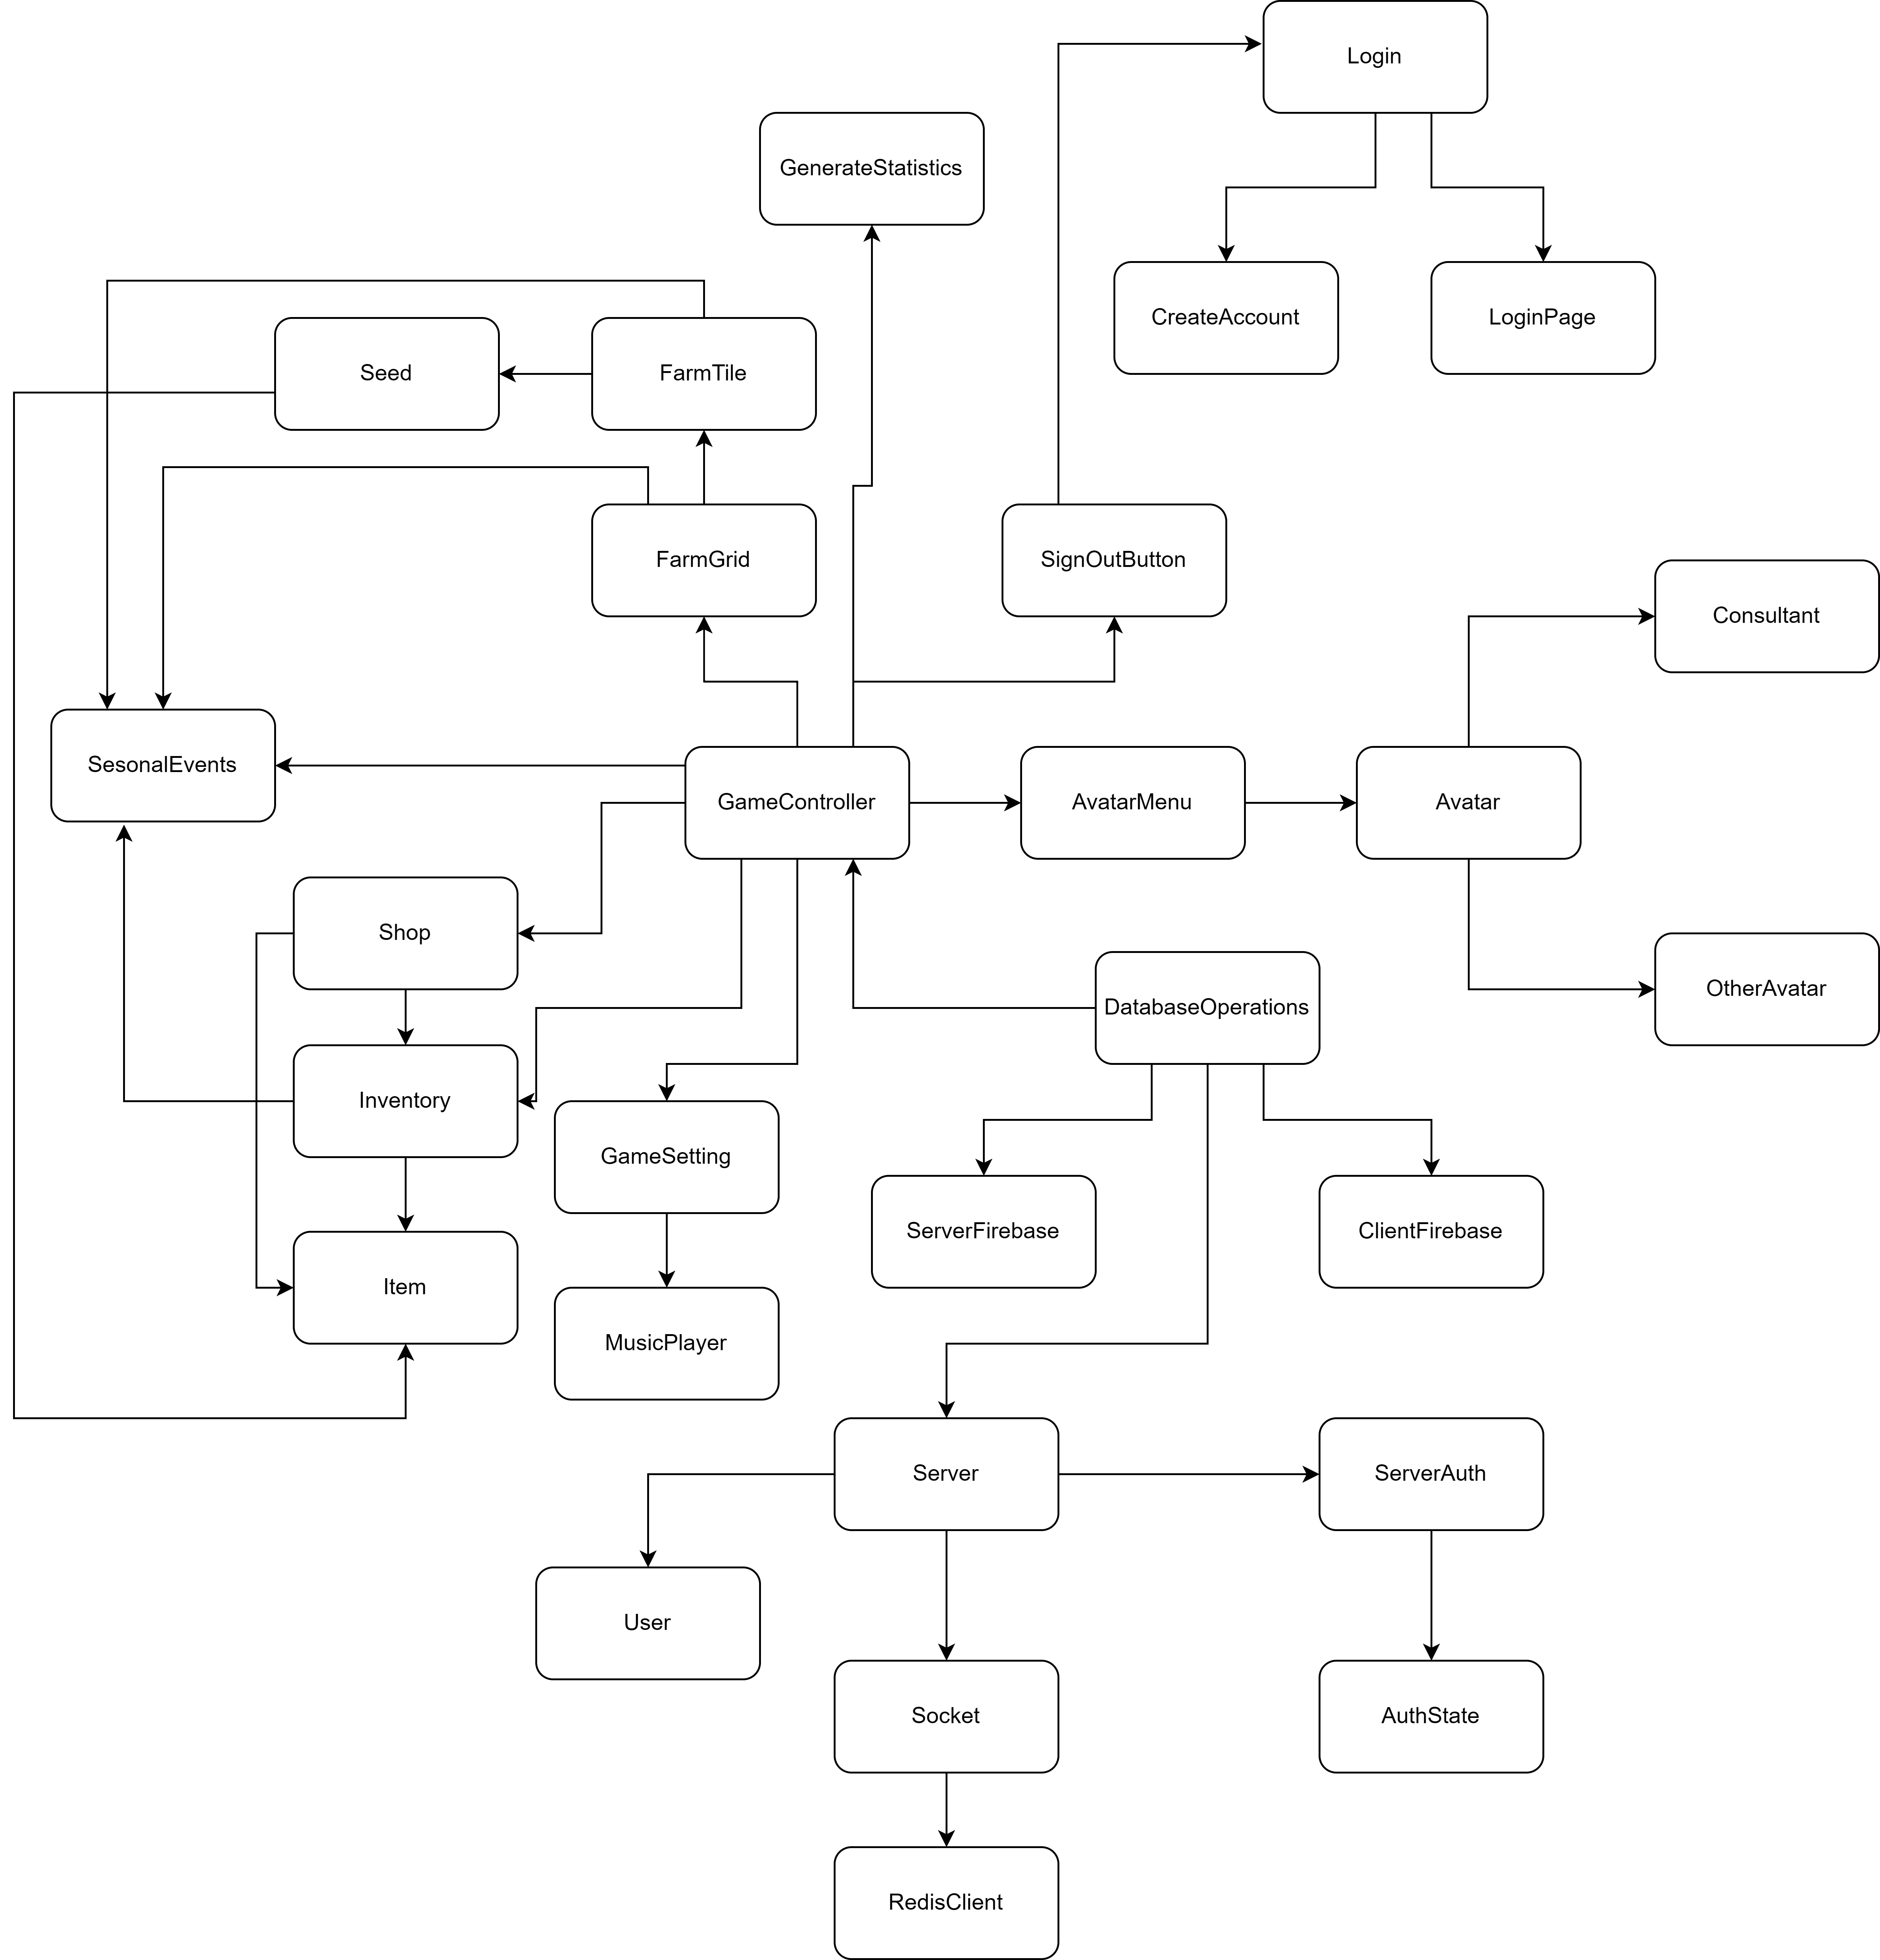
\includegraphics[width=\textwidth]{./capstone_MG_diagram.drawio.png}
\caption{Use hierarchy among modules}
\label{FigUH}
\end{figure}

%\section*{References}

\bibliographystyle {plainnat}
\bibliography{../../../refs/References}

\newpage{}

\end{document}